\documentclass[11pt]{article}

%%%%%%%%%%%%
% Packages %
%%%%%%%%%%%%
\hyphenpenalty=10000
\RequirePackage[normalem]{ulem} %DIF PREAMBLE
\RequirePackage{color}\definecolor{RED}{rgb}{1,0,0}\definecolor{BLUE}{rgb}{0,0,1} %DIF PREAMBLE
\providecommand{\DIFadd}[1]{{\protect\color{blue}\uwave{#1}}} %DIF PREAMBLE
\providecommand{\DIFdel}[1]{{\protect\color{red}\sout{#1}}}    
\usepackage{tocloft}
\renewcommand\cftsecleader{\cftdotfill{\cftdotsep}}
\def\undertilde#1{\mathord{\vtop{\ialign{##\crcr
$\hfil\displaystyle{#1}\hfil$\crcr\noalign{\kern1.5pt\nointerlineskip}
$\hfil\tilde{}\hfil$\crcr\noalign{\kern1.5pt}}}}}
\usepackage{cleveref}
\usepackage{xcolor}
\usepackage{hyperref}
\usepackage{epstopdf}
\usepackage{braket}
\usepackage{upgreek}
\usepackage{caption}
\usepackage{booktabs}
\usepackage{subcaption}
\usepackage{amssymb,latexsym,amsmath,gensymb}
\usepackage{latexsym}
\usepackage{graphicx}
\usepackage{float}
\usepackage{enumitem}
\usepackage{pdflscape}
\usepackage{url}
\usepackage{tikz, calc}
\usetikzlibrary{shapes.geometric, arrows, calc}
\tikzstyle{norm} = [rectangle, rounded corners, minimum width=2cm, minimum height=1cm,text centered, draw=black]
\tikzstyle{arrow} = [thick, ->, >=stealth]

\providecommand{\e}[1]{\ensuremath{\times 10^{#1}}} 
\providecommand{\mb}[1]{\mathbf{#1}}
\providecommand{\mh}[1]{\mathbf{\hat{#1}}}
\providecommand{\bs}[1]{\boldsymbol{#1}} 
\providecommand{\intinf}{\int_{-\infty}^{\infty}}
\providecommand{\fig}[4]{
  % filename, width, caption, label
\begin{figure}[h]
 \captionsetup{width=1.0\linewidth}
 \centering
 \includegraphics[width = #2\textwidth]{#1}
 \caption{#3}
 \label{fig:#4}
\end{figure}
}

\newcommand{\tensor}[1]{\overset{\text{\tiny$\leftrightarrow$}}{\mb{#1}}}
\newcommand{\tunderbrace}[2]{\underbrace{#1}_{\textstyle#2}}
\providecommand{\figs}[7]{
  % filename1, filename2, caption1, caption2, label1, label2, shift
\begin{figure}[H]
\centering
\begin{minipage}[b]{.45\textwidth}
  \centering
  \includegraphics[width=1.0\linewidth]{#1}
  \captionsetup{justification=justified, singlelinecheck=true}
  \caption{#3}
  \label{fig:#5}
\end{minipage}
\hspace{2em}
\begin{minipage}[b]{.45\textwidth}
  \centering
  \includegraphics[width=1.0\linewidth]{#2}
  \vspace{#7em}
  \captionsetup{justification=justified}
  \caption{#4}
  \label{fig:#6}
\end{minipage}
\end{figure}
}
\makeatletter

\providecommand{\code}[1]{
\begin{center}
\lstinputlisting{#1}
\end{center}
}

\newcommand{\crefrangeconjunction}{--}
%%%%%%%%%%%
% Spacing %
%%%%%%%%%%%
% Margins
\usepackage[
top    = 1.5cm,
bottom = 1.5cm,
left   = 1.5cm,
right  = 1.5cm]{geometry}

% Indents, paragraph space
%\usepackage{parskip}
\setlength{\parskip}{1.5ex}

% Section spacing
\usepackage{titlesec}
\titlepacing*{\title}
{0pt}{0ex}{0ex}
\titlespacing*{\section}
{0pt}{0ex}{0ex}
\titlespacing*{\subsection}
{0pt}{0ex}{0ex}
\titlespacing*{\subsubsection}
{0pt}{0ex}{0ex}

% Line spacing
\linespread{1.1}

%%%%%%%%%%%%
% Document %
%%%%%%%%%%%%
\begin{document}
\title{\vspace{-2.5em} Excitation and Detection Efficiency of Ensembles of
  Molecules Under Polarized Illumination \vspace{-1em}} \author{Talon
  Chandler}% and Patrick La Rivi\`ere}
\date{\vspace{-1em}September 19, 2017\\ (Last Updated: \today)\vspace{-1em}}
\maketitle
\section{Introduction}
In these notes I will calculate the excitation and detection efficiencies of
ensembles of molecules as a function of polarizer orientation and microscope
geometry. This work extends the results in the 2017-06-14 notes from single
molecules to ensembles of molecules.

We start by extending the excitation and detection efficiencies to arbitrary
distributions of molecules. Next, we review possible orientation distribution
functions that we can expect real ensembles to follow. Finally, we see how
orientation distributions affect the intensities measured by microscopes.

\section{Intensity Collected From An Arbitrary Distributions of Molecules}
Previously we showed that the excitation efficiency of a single molecule under
incoherent uniform angular illumination is given by
\begin{align}
  \eta_{\text{abs}} &= D\{A + B\sin^{2}{\Theta} + C\sin^{2}{\Theta} \cos{[2 (\Phi - \phi_{\text{exc}}})]\}\label{eq:scalarabs}
\end{align}
where
\begin{subequations}
\begin{align}
  A &= \frac{1}{4} - \frac{3}{8} \cos{\alpha } + \frac{1}{8} \cos^{3}{\alpha }\\
  B &= \frac{3}{16} \cos{\alpha } - \frac{3}{16} \cos^{3}{\alpha }\\
  C &= \frac{7}{32} - \frac{3}{32} \cos{\alpha } - \frac{3}{32} \cos^{2}{\alpha } - \frac{1}{32} \cos^{3}{\alpha}\\
  D &= \frac{4}{3(1 - \cos\alpha)}.
\end{align}\label{eq:coefficients}%
\end{subequations}
If the detector does not use a polarizer then the detection efficiency is given by
\begin{align}
  \eta_{\text{det}} = 2(A + B\sin^2\Theta).
\end{align}


\DIFdel{If an ensemble of independent fluorescent molecules is illuminated then the
absorption efficiency of the ensemble is}
\begin{align}
  \DIFdel{\eta_{\text{abs}} = \int_{\mathbb{S}^2}d\mh{r} f(\mh{r}) \eta_{\text{abs}}^{\text{single}}} \label{eq:ensemble}%
\end{align} 
\DIFdel{where $f(\mh{r})$ is the orientation probability distribution function of the
fluorophores. For equation \ref{eq:ensemble} to be true the fluorophores must
absorb light independently---no homo-FRET or coherence effects.}

\DIFdel{Similarly, the detection efficiency of an ensemble is}
\begin{align}
  \DIFdel{\eta_{\text{det}} = \int_{\mathbb{S}^2}d\mh{r} f(\mh{r}) \eta_{\text{det}}^{\text{single}}} \label{eq:ensemble_det}%
\end{align} 
\DIFdel{which is only true if the fluorophores emit light independently. If the detector
  uses a polarizer then $\eta_{\text{det}}^{\text{single}}$ is given by equation 2 with $D = 1$ (see Fourkas \cite{fourkas2001}).}

The detected intensity is proportional to
\begin{align}
  \DIFadd{I \propto I_{\text{out}}\int_{\mathbb{S}^2}d\mh{r} f(\mh{r}; \hat{\bs{\mu}}, \kappa) \eta_{\text{exc}}(\mh{r}) \eta_{\text{det}}(\mh{r})} \label{eq:ensemble_intensity}%
\end{align}
\begin{align}
  \DIFdel{I \propto I_{\text{out}}\eta_{\text{abs}}\eta_{\text{det}}. }
\end{align}
Our goal is to estimate the parameters of the ensemble distribution ($\Theta$,
$\Phi$, $\kappa$) and the total output intensity (proportional to the number of
molecules in the distribution $N$) from the intensity measurements. \DIFdel{If we can
estimate the number of photons each fluorophore emits (from a datasheet or a
separate experiment), then we can estimate $N$ directly. If this information is
not available, we will estimate a number that is directly proportional to $N$.}

\DIFadd{Note that equation 6 integrates the intensity contributions from each
  fluorophore. The previous expressions (equations 4, 5, and 7) integrate the
  efficiencies which is incorrect.}

Note that equation \ref{eq:ensemble_det} is much more computationally expensive
than the single molecule efficiencies that I've implemented previously. The
double integrals do not have closed form solutions, so I am using a numerical
integration scheme---Gausse-Legendre adaptive quadrature methods implemented in
QUADPACK and called from \texttt{scipy}. These methods allow us to easily trade
speed for accuracy.

\section{Axial Distributions On The Sphere}
In this section we will review several orientation probability distribution functions. 

The \textbf{Von Mises-Fisher distribution} is given by
\begin{align*}
  f(\mh{r}; \bs{\hat{\mu}}, \kappa) = \frac{\sqrt{\kappa}}{(2\pi{})^{3/2}I_{1/2}(\kappa)}\text{exp}\{\kappa \bs{\hat{\mu}}^T\mh{r}\}
\end{align*}
where $I_{1/2}$ denotes the modified Bessel function of the first kind. The Von
Mises-Fisher distribution is rotationally symmetric about $\bs{\hat{\mu}}$, but
it is not antipodally symmetric. Therefore, the Von Mises-Fisher distribution is
not an appropriate choice for modeling axial data.

\fig{../figures/vonmises.pdf}{1.0}{Von Mises-Fisher distributions with constant $\bs{\hat{\mu}}$ and varying $\kappa$. }{vonmises}

The \textbf{Watson distribution} \cite{sra2007modeling, jupp} is given by
\begin{align*}
  f(\mh{r}; \bs{\hat{\mu}}, \kappa) = \frac{1}{4\pi{}_1F_1\left(\frac{1}{2}, \frac{3}{2}, \kappa\right)}\text{exp}\{\kappa (\bs{\hat{\mu}}^T\mh{r})^2\}
\end{align*}
where ${}_1F_1$ denotes a confluent hypergeometric function. The Watson
distribution is antipodally symmetric ($f(\mh{r}) = f(-\mh{r})$) and
rotationally symmetric about $\bs{\hat{\mu}}$. The parameter $\kappa$ is a
concentration parameter---when $\kappa$ is large and positive the distribution
is concentrated near $\mu$, when $\kappa$ is large and negative the distribution
is concentrated near the great circle orthogonal to $\bs{\hat{\mu}}$, and when
$\kappa$ is small the distribution is uniform. $\bs{\hat{\mu}}$ is a unit vector
which can be specified using two angles, so the Watson distribution is a 3
parameter distribution.

The Watson distribution is (1) antipodally symmetric, (2) rotationally symmetric
about a single axis, and (3) smooth, so we think it is a good distribution to
describe distributions of molecules in biological samples. The Watson
distribution has also been used as a model for paleomagnetic data (orientations
of the magnetic axis in rocks) \cite{Love2007}, MRI diffusion tensor imaging
data \cite{Jespersen2012}, and microphone array directionality data
\cite{alex}. We will use the Watson distribution as a model for fluorophores for
the remaining sections of these notes.

\fig{../figures/watson.pdf}{1.0}{Watson distributions with constant
  $\bs{\hat{\mu}}$ and varying $\kappa$. }{watson}

For completeness, the \textbf{Bingham distribution} \cite{sra2007modeling, jupp}
is a generalized version of the Watson distribution that allows for
distributions that are not rotationally symmetric about a single axis. The
Bingham distribution is given by
\begin{align}
  f(\mh{r}; \bs{\hat{\mu}}, \kappa) = \frac{1}{4\pi{}_1F_1\left(\frac{1}{2}, \frac{3}{2}, \mb{K}\right)}\text{exp}\{\mh{r}^T\mb{K}\mh{r}\}
\end{align}
where ${}_1F_1$ is denotes a confluent hypergeometric function with a matrix
argument. The matrix $\mb{K}$ has three free parameters (two eigenvalues and a
choice of principal axis), so the Bingham distribution is a 5 parameter
distribution.

\section{Example Results}

Figure \ref{fig:single-frame} shows representative examples of intensity
measurements collected from Watson-distributed fluorophores. Note how the
intensity pattern changes as $\kappa$ changes. For large $\kappa$, we recover
the case of single fluorophores and there is a concentrated set of orientations
with high intensity. As $\kappa$ decreases, the set of orientations with
high total efficiency grows until $\kappa = 0$ and the total efficiency is
independent of $\bs{\hat{\mu}}$ (this is because the mean orientation is
meaningless for a uniform distribution). When $\kappa < 0$ the total efficiency
is high in a ring of orientations.

\begin{figure}[h]
 \captionsetup{width=1.0\linewidth}
 \centering
 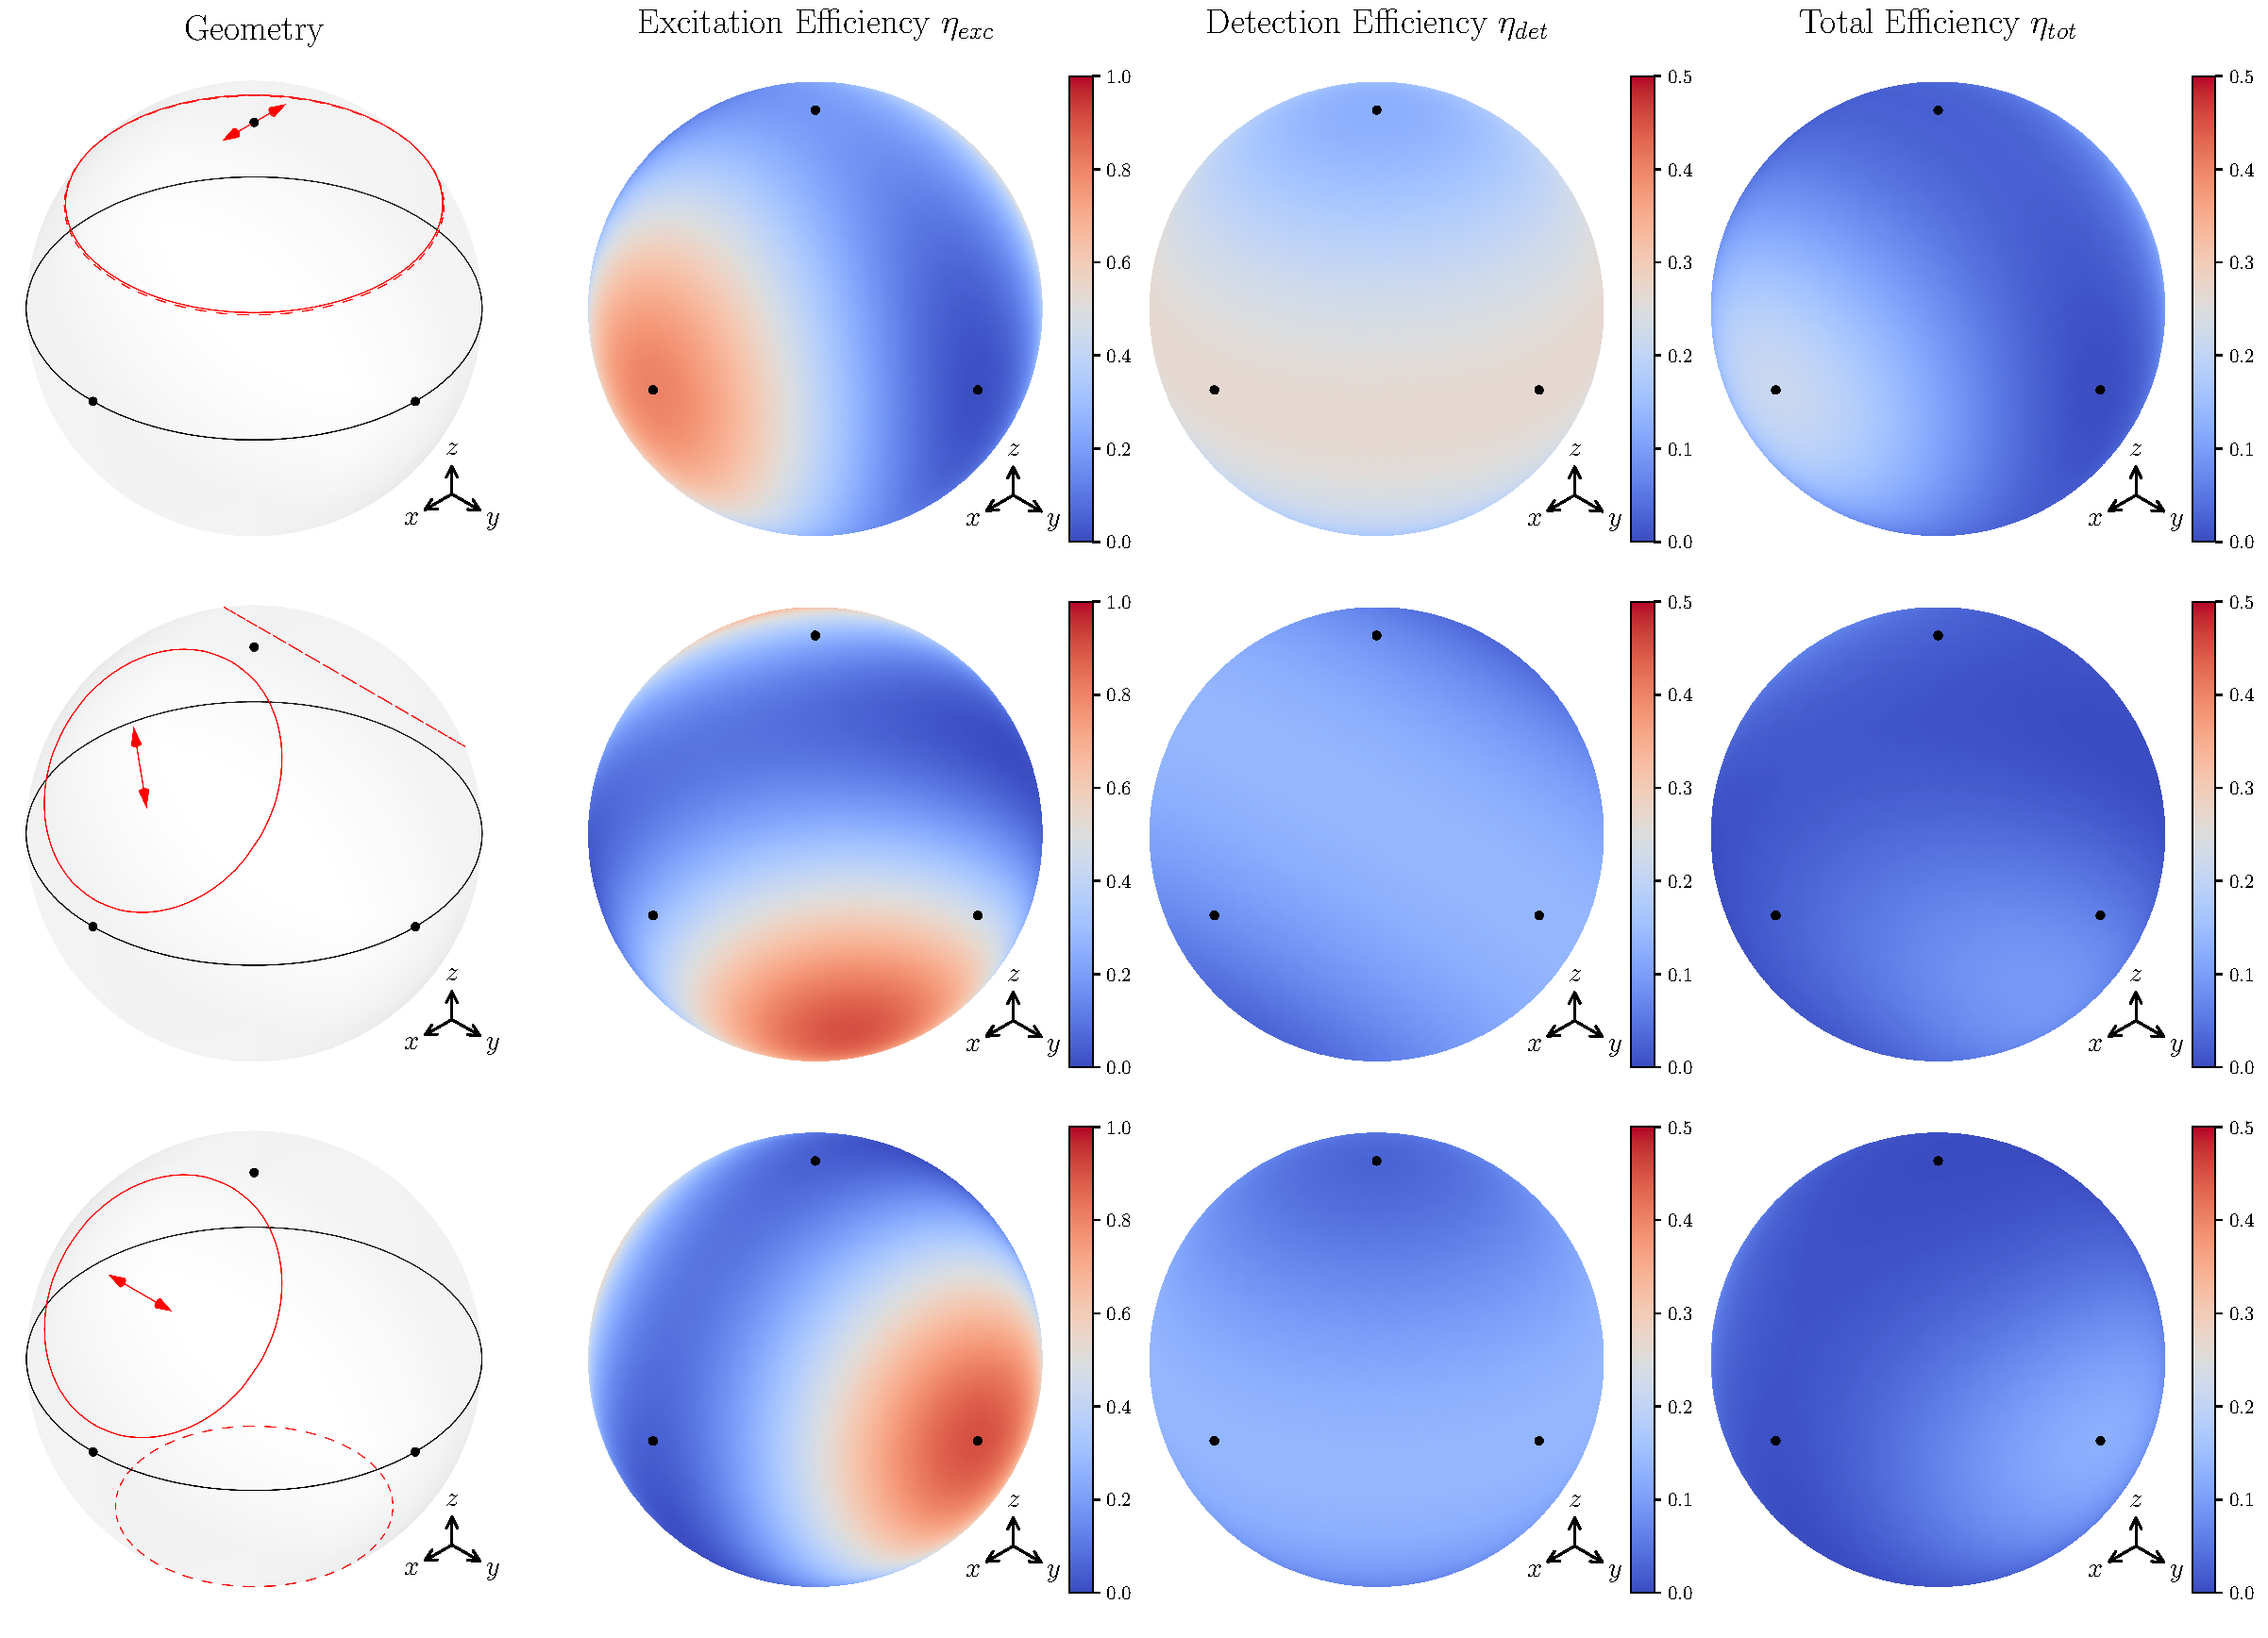
\includegraphics[width = 0.8\textwidth]{../figures/single-frame.pdf}
 \caption{\DIFadd{Replaced figure. Shows intensity instead of ``ensemble
     efficiencies''.} Representative examples of ensemble intensity
   measurements. Black dots indicate where the Cartesian unit vectors intersect
   the unit sphere. \newline \newline \textbf{Columns left to right:} 1)
   fluorophore distributions with $\bs{\hat{\mu}} = \mb{\hat{z}}$ and varying
   $\kappa$; 2) microscope geometry schematics---all cases use two 0.8 NA
   objectives in a diSPIM geometry with polarized illumination and unpolarized
   detection 3) \DIFadd{the measured intensity as a function of $\bs{\hat{\mu}}$,
     see equation \ref{eq:ensemble_intensity}}. \DIFdel{the absorption efficiency as a
     function of $\bs{\hat{\mu}}$, see equation \ref{eq:ensemble_intensity}; 3)
     the detection efficiency as a function of $\bs{\hat{\mu}}$, see equation
     \ref{eq:ensemble_det}; (4) the total efficiency, the product of the
     absorption and detection efficiencies. \textbf{Note:} The last three
   columns do not use the same scale.}}
 \label{fig:single-frame}
\end{figure}

% \fig{../figures/single-frame.pdf}{1.0}{\DIFadd{Replaced figure. Shows intensity
%     instead of ``ensemble efficiencies''.} Representative examples of ensemble
%   intensity measurements. Black dots indicate where the Cartesian unit vectors
%   intersect the unit sphere. \newline \newline \textbf{Columns left to right:}
%   1) fluorophore distributions with $\bs{\hat{\mu}} = \mb{\hat{z}}$ and varying
%   $\kappa$; 2) microscope geometry schematics---all cases use two 0.8 NA
%   objectives in a diSPIM geometry with polarized illumination and unpolarized
%   detection 3) \DIFadd{the measured intensity as a function of $\bs{\hat{mu}}$,
%     see equation \ref{eq:ensemble}}. \DIFdel{the absorption efficiency as a
%       function of $\bs{\hat{\mu}}$, see equation \ref{eq:ensemble_intensity}; 3) the
%       detection efficiency as a function of $\bs{\hat{\mu}}$, see equation
%       \ref{eq:ensemble_det}; (4) the total efficiency, the product of the
%       absorption and detection efficiencies.} \textbf{Note:} The last three
%     columns do not use the same scale.}{single-frame}

\section{Computation Time Estimates}
A function evaluation for the intensity collected from a single fluorophore
\textbf{currently} takes $\sim$ 0.1 ms.

To calculate the intensity collected from a distribution of fluorophores we need
to repeat this calculation for each fluorophore orientation. Empirically,
$\sim 500$ orientations bounds the error on the integral below 1\%, so the full
calculation takes $\sim 50$ms.

We're planning to implement a Fisher scoring algorithm that acts on the data
from each voxel to estimate 4 parameters: the orientation distribution
($\Theta$, $\Phi$, $\kappa$) and the number of fluorophores $N$ (or a parameter
that is proportional to $N$). The algorithm (1) computes the Fisher information
matrix at a starting guess which takes 5 function evaluations (a central point
and 4 derivative directions) which takes $\sim 0.25\ \text{s}$, (2) updates its
guess (cheap), then (3) recomputes the Fisher information matrix until
convergence. It's difficult to guess the number of iterations we will require
for convergence, but let's say we can get it down to 10 iterations ($\sim$ 2.5
s).

The data set we took this summer has $\sim 150\times 150\times 800 \approx 2\e{7}$
useful voxels which will take $\sim5\e{7} \text{s} = 1.5\ \text{y}$.

There are still plenty of places we can save time. In approximate order of ease:
\begin{enumerate}
\item Move the function evaluations from Python to C. This shouldn't take much
  more than a day, and forums report a 3-10$\times$ improvement.
\item Optimize the integration method to reduce the number of function
  evaluations. Empirically, when $\kappa$ is small we need fewer that 500
  function evaluations for the integration to have a 1\% error.
\item Bin voxels ($2\times2\times2$ binning gives $8\times$ speedup,
  $3\times3\times3$ gives $27\times$ speedup).
\item Process voxels in parallel on the GPU (10-1000$\times$ speedup)
\end{enumerate}

All of these improvements together will (conservatively) put the reconstruction time at $\sim 1\ \text{day}$, and likely much faster.
\bibliography{report}{}
\bibliographystyle{unsrt}

\end{document}

